\section{XP}

\begin{frame}
\begin{block}{}
	 \begin{figure}[!htb]
			\centering	  				
			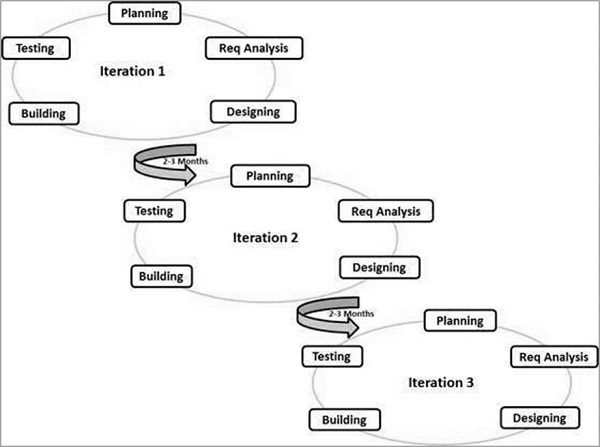
\includegraphics[height=7cm, width = 11cm]{./pic/sdlc_agile_model.jpg}
			\caption{Etapas da metodologia XP \cite{TUTORIALSPOINT}}
			\label{fig_cascata}
		\end{figure}
\end{block}
\end{frame}


\begin{frame}
\begin{block}{Detalhes}
	 \begin{itemize}
			\item Ciclo de iteração curto (15 dias, 1 mês):

			\item Escrever histórias de usuário
			
			\item Escrever os testes de aceitação pelo cliente
			
			\item Priorizar as histórias junto com o usuário
			
			\item Estabelecer um MVP (produto mínimo que agrega valor para o cliente)
			
			\item Codificar
			
			\item Testar
			
			\item Entregar para o cliente
			
			\item Próximo ciclo!
			
			\item Não temos a definição perfeita do projeto todo, por isso priorizamos apenas no que conhecemos e sabemos.

	 \end{itemize}
\end{block}
\end{frame}

\begin{frame}
\begin{block}{Trade-off}
	 \begin{itemize}
			\item É mais complexo o gerenciamento e compreensão, afinal considera a mudança constante do negócio.

			\item É realista, considera mudanças, entrega valor rápido, menos propenso ao retrabalho.
			
			\item Caso a história não seja usada, o negócio mudou, por exemplo, o tempo gasto nela foi menor que o cascata pois trabalhamos com pequenos ciclos de interação.
			
			\item Não existe: “Vamos fazer toda a documentação”, ela é feita apenas para os pontos relevantes da história.
			
			\item Programação em pares.
			
			\item Cliente presente (de alguma forma mesmo que não fisicamente). Explicar meu caso de cliente ausente na PagSeguro e Itaú.

	 \end{itemize}
\end{block}
\end{frame}

\begin{frame}
\begin{block}{Roles}
	 \begin{itemize}
			\item Desenvolvedor – quem irá desenvolver o game

			\item Coach – é o técnico que garante a aplicação da cultura ágil.
			
			\item Testador – quem irá testar o game
			
			\item Cliente – Quem informa os desafios de negócio que devemos resolver
			
			\item Cleaner – Refatora o código e cobra a equipe toda para manter a limpeza do mesmo
			
			\item Tracker – Coleta as métricas do projeto
			
			\item Gerente – Cobra as entregas do projeto

	 \end{itemize}
\end{block}
\end{frame}

\begin{frame}
\begin{block}{Visão}
	 \begin{itemize}
			\item Time multidisciplinar e coeso

			\item Time sabe se gerenciar sozinho, gerente é um facilitador
			
			\item Time fisicamente próximo
			
			\item Reuniões de revisão para avaliar onde podemos melhorar (Não caçar as bruxas!)
			
			\item Cliente presente
			
			\item Liberação frequente de pequenas entregas (Mas professor... Em games isso é viável?)
			
			\item Faça POC e não reaproveite o código da POC! Normalmente é um código inicial para aprendizagem de baixa qualidade

	 \end{itemize}
\end{block}
\end{frame}


\begin{frame}
\begin{block}{Exercício}
	 \begin{itemize}
		\item Vamos escrever uma história de usuário, no papel, para desenvolver o jogo: “Age of Empires”. Cada aluno escreverá uma história distinta.

		\item Exemplo de história de usuário:
		
		\item Eu como {USUARIO DO SISTEMA} gostaria de ter a funcionalidade {FUNCIONALIDADE} para que  me permita  {OBJETIVO} pois isso agrega valor para meu negócio da seguinte forma {AGREGAÇÂO DE VALOR}
	 \end{itemize}
\end{block}
\end{frame}

\begin{frame}
\begin{block}{Exercício Priorização}
	 \begin{itemize}
		\item Agora vamos priorizar as histórias:

		\item O que agrega mais valor para o cliente primeiro?
		
		\item O que queremos garantir que ele já vá testando antes?
		
		\item Quais histórias estão incertas?
		
		\item O que podemos deixar para depois?
		
		\item Quais histórias são imprescindíveis para nós desenvolvermos?
	 \end{itemize}
\end{block}
\end{frame}

\begin{frame}
\begin{block}{XP x Cascata}
	 \begin{itemize}
		\item Vamos simular um projeto de game com as duas metodologias e avaliar qual delas é mais útil para a realidade dos games.

		\item Nosso contexto agora é o jogo: “World of Warcraft”.
		
		\item Os alunos serão os programadores e testadores.
		
		\item O professor será o cliente e gerente, simulando duas pessoas distintas.
	 \end{itemize}
\end{block}
\end{frame}